\documentclass[reprint,aps,prl,twocolumn,superscriptaddress,groupedaddress]{revtex4-2}
\usepackage{CJKutf8}
\usepackage[utf8]{inputenc}


\usepackage[final]{graphicx}
\usepackage[hidelinks]{hyperref}
\usepackage{bm,physics,amsmath,amssymb,xcolor}
\usepackage[normalem]{ulem}

\usepackage{centernot}
\usepackage{braket}
\usepackage{tabularx}
\usepackage{booktabs}
\usepackage{pifont}
\usepackage{colortbl}
\usepackage{amsthm}
\usepackage{soul}
\usepackage{epsfig}

\setcounter{secnumdepth}{4}
\usepackage{titlesec}

\newcommand{\eomo}{$E_1$-$M_1$}
\newcommand{\eoet}{$E_1$-$E_2$}
\newcommand{\etet}{$E_2$-$E_2$}
\newtheorem{theorem}{Theorem}
\newtheorem*{remark}{Theorem}
\definecolor{CL_Yellow}{HTML}{E69E5B}
\colorlet{LightYellow}{CL_Yellow!25}
\definecolor{CL_Pink}{HTML}{9E5BE6}
\colorlet{LightPink}{CL_Pink!25}
\definecolor{CL_Green}{HTML}{9EE65B}
\colorlet{LightBlue}{CL_Green!25}
\newcommand{\cg}[3]{C^{#1}_{#2;#3}}
\newcommand{\ii}{\mathrm{i}}

\newcommand{\correction}[2]{\textcolor{red}{\sout{#1}} \textcolor{blue}{#2}}
\newcommand{\hide}[1]{}

\usepackage{printlen}
\makeatletter
\edef\textFontName{\fontname\csname
  \f@encoding/\f@family/\f@series/\f@shape/\f@size\endcsname}
\edef\mathFontName{\fontname\textfont0}
\edef\mathLetterFontName{\fontname\textfont1}
\makeatother
\newcommand{\printsizes}{
    \uselengthunit{in}~\\
    textwidth: \printlength{\textwidth}\\
    linewidth: \printlength{\linewidth}\\
    text height: \printlength{\textheight}\\
    font name: \textFontName \\
    font size: \the\fontdimen6\font\relax
}
\begin{document}
\begin{CJK*}{UTF8}{gbsn}
\title{振转螺旋二色性的自下而上分析}
\author{Mateja Hrast}
\email[]{mateja.hrast@ist.ac.at}
\affiliation{奥地利科学技术研究所(ISTA),克洛斯特新堡校区1号,3400}
\author{Georgios M. Koutentakis}
\email{georgios.koutentakis@ist.ac.at}
\affiliation{奥地利科学技术研究所(ISTA),克洛斯特新堡校区1号,3400}
\author{Mikhail Maslov}
\email{mikhail.maslov@ist.ac.at}
\affiliation{奥地利科学技术研究所(ISTA),克洛斯特新堡校区1号,3400}
\author{Mikhail Lemeshko}
\email{mikhail.lemeshko@ist.ac.at}
\affiliation{奥地利科学技术研究所(ISTA),克洛斯特新堡校区1号,3400}
\date{\today}
\begin{abstract}
螺旋二色性(Helical Dichroism, HD)是一种利用光轨道角动量(Orbital Angular Momentum, OAM)解析分子手性的新兴方法。本研究突破传统HD理论的假设框架,基于分子对称性与转动本征态,构建了严格的HD分析理论体系。通过推导转动选择定则,我们明确论证了HD现象仅源于光的自旋-轨道耦合效应,即使对于不携带远场OAM的光束亦然。研究成果细化了观测HD的实验条件,不仅为已有实验结果提供了理论阐释,更为未来基于结构光的手性传感设计提供了重要指导。
\end{abstract}
\maketitle
许多具有生物和化学重要性的分子以手性对形式存在——两种不可重叠的镜像版本称为对映体。分离对映体的能力对于制药和农用化学品工业至关重要\cite{MAIER2001}。这一现象最典型的例证莫过于甲基苯丙胺分子:其R-对映体是有效的鼻充血缓解剂,而S-对映体则是导致成瘾流行的精神活性药物~\cite{barkholtz2023}。巨大的经济价值推动了手性分子不对称合成的研究,例如通过立体选择性或生物催化,或使用手性辅助剂\cite{Brown1989}。然而,这些先进合成技术仍需进一步完善,且需要通过立体选择性过程评估对映体纯度。这一关键步骤目前仍面临技术挑战,现有化学方法各自存在成本高、耗时长、适用性有限或可靠性不足等问题\cite{qian2023}。本文从化学物理交叉视角出发,探索通过光-物质相互作用评估对映体纯度的新途径。得益于光学物理的快速发展\cite{Koch2019},该方法有望为手性识别提供经济高效且高度可控的解决方案。

数十年来,左旋与右旋圆偏振光吸收差异(即圆二色性CD)\cite{deutsche1970,Holzwarth1974}一直被用于手性介质光谱学研究\cite{Miles2021}。然而,圆二色性依赖于光的自旋角动量这一有限资源。与此同时,Allen等人\cite{Allen1992}的开创性工作揭示:除自旋外,光还可携带轨道角动量(OAM)。与自旋不同,光束携带的OAM量子数原则上没有上限。具有螺旋波前的OAM光束因其手性结构与物质手性相匹配的特性,为立体选择性应用提供了前所未有的可能性。

这种探索催生了利用OAM诱导过程检测对映体纯度的具体方案,特别是以螺旋二色性(HD)\cite{ANDREWS2004,Ye2019,Li2021}形式呈现的技术,其被认为较CD有显著改进\cite{Ye2019,Li2021}。Forbes与Andrews的奠基性理论工作\cite{Forbes2018,Forbes2019,Forbes2021}系统分析了光-物质相互作用多极展开项的对称性,明确指出电偶极-磁偶极(\eomo)、电偶极-电四极(\eoet)及电四极-电四极(\etet)项可作为手性识别因子。他们推导了\eoet跃迁振幅与分子多极矩的关系表达式,但未尝试从分子转动态角度进行量化。实验方面,早期研究未能观测到HD信号\cite{Araoka2005,Loeffler2011},但近期实验声称实现了观测\cite{Rusak2019,Zhang2020,Rouxel2022,Begin2023,Jain2023}。不过这些实验装置极为复杂,且尽管理论认为强聚焦是必要条件\cite{Forbes2019},目前尚未有研究阐明观测到二色性的物理机制。

本研究通过揭示转动振动光谱中HD产生的条件填补了这一空白。我们首先概述基于分子多极矩的手性检测方法,推导\eoet二色性观测的对称性要求。利用新近发展的分子-光相互作用哈密顿量\cite{Maslov2024,Maslov_Thesis},我们推导出\eoet项诱导的转动振动跃迁选择定则。分析表明,傍轴拉盖尔-高斯(LG)光束无法产生真正的HD(即源于OAM转移的HD)。特别地,强聚焦至关重要——因为光的自旋-轨道耦合(SOC)\cite{Bliokh2015}能使OAM转移至手性分子,产生傍轴近似下不存在的HD贡献。更有趣的是,我们发现即使不携带远场OAM的高斯光束,在强聚焦条件下也能产生HD信号。这些发现完善了转动振动光谱中HD的理论基础,为未来利用结构光进行对映体选择性实验和技术设计提供了指导。

现有对映体敏感方法多基于分子多极矩分析。标准手性检测方法——(振动)圆二色性涉及\eomo项,已有详尽研究\cite{Stephens1985,BUCKINGHAM1987,Mun2019,Lovesey2019}。其原理在于:手性分子的电偶极矩作为矢量在镜像反射下变号,而作为赝矢量的磁偶极矩保持不变。两者共存表明分子缺乏镜面对称性(严格说是非真旋转轴),即具有手性。该方法要求分子对称性至少允许一个非零偶极矩,使其能探测多种对称群的手性分子。但\eomo项二色性仅取决于场强,这促使人们寻求可通过场结构增强二色性的替代方案。

相位敏感微波三波混频技术\cite{Patterson2013,Patterson2013PRL}即为一例,其利用偶极矩乘积$d_xd_yd_z\neq 0$作为手性判据\cite{Patterson2013,Ordonez2018,Ayuso2022}。对称性分析表明,仅完全不对称($C_1$)手性分子满足此条件。我们研究则探索了另一方向——源于分子电偶极矩与电四极矩的手性条件。\eoet项诱导的二色性可通过场结构增强,使其成为未来对映体敏感技术的理想候选。近期研究还提出磁偶极-磁四极($M_1$-$M_2$)耦合可作为HD来源,其对称性与\eoet项等效\cite{Ji2024}。但此类高阶项(如\etet)因多极展开中跃迁概率过低而难以检测。\\
本文余下部分将重点分析源自\eoet 项的二色性特征。基于简单的点电荷模型,我们推导出以下条件(证明详见补充材料\footnote{参见补充材料,其中包含参考文献\cite{Maslov2024,Maslov_Thesis,Lax1975,Bliokh2015,Bliokh2023}}):\\
\textit{若在主轴坐标系中,对于互异的$\mu, \nu, \rho \in \{x,y,z\}$坐标,偶极矩与四极矩的乘积$d_{\mu}Q_{\nu \rho} \neq 0$,则该分子具有手性。}\\
该条件迄今一直与螺旋二色性(HD)相关联\cite{ANDREWS2004,Forbes2018}。然而,本研究表明:即使光场未向分子内自由度传递轨道角动量(OAM),该条件同样能产生鉴别效应。本文中HD特指伴随OAM转移的二色性效应,而即便使用携带OAM的光束也不发生OAM转移的二色性则称为圆二色性(CD)。

表~\ref{tab:chiral_multipole_dofs}总结了\eoet 项可诱导二色性的手性点群。在纯转动光谱中,仅需考虑分子的永久多极矩;而在振转光谱中,振动跃迁会改变分子态对称性,因此需根据不可约表示$V$分析终态振动能级的变换性质,这使得更多手性群可被检测。表~\ref{tab:chiral_multipole_dofs}列出了各手性点群中呈现二色性的$V$表示。
\begin{table}[ht!]
    \centering
    \caption{所有可能手性点群的旋转光谱与旋转振动光谱中的\eoet~手性特征。对于旋转振动光谱,我们还给出了与非零手性特征相关联的振动模式不可约表示。}
     \setlength\tabcolsep{3pt}
\begin{tabular}{p{70pt} | c c c c c c c c c c}
\toprule
     Point group     & $C_1$ & $C_2$ & $C_{n\geq 3}$ & $D_2$ & $D_{n\geq 3}$ & $T$ & $O$ & $I$ \\ \midrule
     Rotational      & \textcolor{black}{\ding{52}} & \textcolor{black}{\ding{52}}& \textcolor{red}{\ding{56}}  & \textcolor{red}{\ding{56}}  & \textcolor{red}{\ding{56}}  & \textcolor{red}{\ding{56}}  & \textcolor{red}{\ding{56}}  & \textcolor{red}{\ding{56}} \\
     Ro-vibrational  & $A$ & $A$, $B$ & $E_1$ & $B_{1, 2, 3}$ & $E_1$ & $T$ & \textcolor{red}{\ding{56}} & \textcolor{red}{\ding{56}} \\
     \bottomrule
\end{tabular}
     \label{tab:chiral_multipole_dofs}
 \end{table}
如表\ref{tab:chiral_multipole_dofs}所示,\eoet 项仅能通过保持分子对称性的跃迁(纯转动及平凡表示$A$的振转跃迁)识别$C_1$和$C_2$对称性的手性分子。鉴于已知手性分子多为$C_1$对称(即不对称陀螺分子)\cite{Bernath},本文研究范围限定于此。

不对称陀螺转子哈密顿量的本征态可用转动基矢$\ket{J,M,K}$表示\cite{Bernath}:
\begin{equation}
    \ket{J_{N_p,N_o}(M)}=\sum_KC_K\ket{J,M,K}.
    \label{basisChange}
\end{equation}
其中$J$为总角动量量子数,$M$和$K$分别为${\bm J}$在实验室量子化轴和本体固定主轴上的投影。不对称陀螺指标$N_p$与$N_o$是纯长椭球/扁椭球解中$K$的极限值,并非好量子数。由于量子数$J$和$M$不受基变换\eqref{basisChange}影响,我们进一步推导转动基矢$| J, M, K \rangle$内电偶极($E_1$)与电四极($E_2$)跃迁的选择定则。

初始态$i=\ket{J,M,K}$至终态$f=\ket{J,M',K'}$的分子转动跃迁速率可通过文献\cite{Maslov2024,Maslov_Thesis}中的光-物质相互作用哈密顿量计算,其跃迁振幅为:
\begin{equation}
    \mathcal{M}_{i\to f}=\sum_{lm\mu}\mathcal{I}^{\text{vib}; l,\mu}\,\mathcal{I}^{\text{CM}; l,m}\,\mathcal{I}^{\text{rot}; l,m,\mu,\sigma}_{J,M,K,J,M',K'}\,,
    \label{eq_transition_matrix}
\end{equation}
式中$l=0$和$l=1$分别对应偶极与四极跃迁,$m = 0, \pm 1, \dots, \pm l$表示传递给分子的OAM,$\mu = 0, \pm 1, \dots, \pm (l+1)$涵盖球基下所选多极矩的所有分量,$\sigma =0, \pm 1$为光的偏振分量。振动项$\mathcal{I}^{\text{vib}; l,\mu}$与质心项$\mathcal{I}^{\text{CM}; l,m}$分别参数化分子与光的特性。本文重点关注决定角动量选择定则的转动跃迁振幅$\mathcal{I}^{\text{rot};l,m,\mu,\sigma}_{J,M,K,J,M',K'}$,其总结于表~\ref{SelectionRules}。
\begin{table}[ht!]
    \centering
    \begin{tabular}{c c}\hline
    \toprule
        \textbf{$E_1$ transition} & \textbf{$E_2$ transition}  \\
        \midrule
        $\Delta J\leq 1$ &  $\Delta J\leq 2$ \\
        $\Delta M=-\sigma$ & $\Delta M=m-\sigma$ \\
        $\Delta K=\pm\mu$ & $\Delta K=\pm\mu$ \\
        $J=0\not\to J'=0$ &  (see \cite{Note1}\\
        $\ket{J,0,K}\not\to\ket{J,0,K'}$ &  for details)\\
    \bottomrule
\hline
    \end{tabular}
    \caption{电偶极子 ($E_1$) 与四极子 ($E_2$) 跃迁在转动态 $\ket{J,M,K}$ 之间的选择定则。关于禁戒跃迁的详细信息请参阅 \cite{Note1}。}
    \label{SelectionRules}
\end{table}
可以证明$\mathcal{I}^{\rm rot; l, m, \mu, \sigma}_{J, M, K, J', M', K'} \propto C^{J',M'}_{l+1, m-\sigma; J, M}$ \cite{Maslov2024,Maslov_Thesis},其中$C^{J, M}_{j_1, m_1, j_2, m_2}$为克莱布什-戈尔丹系数(推导过程见补充材料\cite{Note1})。要实现电偶极-电四极(\eoet)跃迁,所选态之间必须同时允许$E_1$($l=m=0$)和$E_2$($l = 1$,$m = 0, \pm 1$)跃迁。对于具有确定偏振$\sigma$的光束,这仅对不携带轨道角动量(OAM)的$m = 0$分量可能实现(见表~\ref{SelectionRules})。由此我们得到本工作的第一个关键结论:源于傍轴光束\eoet~项的二色性不应与螺旋二色性(HD)关联,因为此时分子未获得OAM。此外,这种二色性甚至在平面波情况下也存在,因此与光场结构或螺旋性完全无关。

这引出一个问题:当发生OAM转移时,\eoet~项能否产生HD?下文将证明在非傍轴光束情况下可以实现这种机制。图~\ref{fig:gridJ1}展示了不对称陀螺分子转动本征态间允许的偶极跃迁(红色方框)与四极跃迁(蓝色方框)。为清晰起见,此处仅显示部分本征态,完整图谱($J\leq 2$)见\cite{Note1},但其定性特征与此一致。

\begin{figure}[ht!]
    \centering
    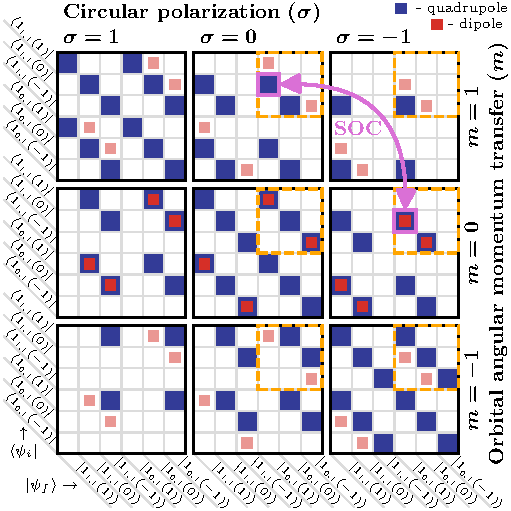
\includegraphics[width=\linewidth]{Figure1.pdf}
    \caption{不对称陀螺哈密顿量本征态之间允许的偶极跃迁(红色方框)与四极跃迁(蓝色方框)。各子图列表示光束的不同圆偏振态,子图行表示光束可传递给分子内转动的轨道角动量数值。紫色圆圈展示自旋-轨道耦合产生\eoet~项并传递轨道角动量的示例。橙色方框标明了实验中会叠加的跃迁,如图\ref{fig:profiles}所示。}
    \label{fig:gridJ1}
\end{figure}
图~\ref{fig:gridJ1}的三列对应不同光束偏振态,三行对应不同OAM转移量子数$m$。如文献\cite{Maslov2024,Maslov_Thesis}所示,电偶极跃迁不转移OAM,故仅出现在$m=0$行(但在$m=\pm 1$行仍作对比展示)。相反,电四极跃迁可转移最多一个OAM量子($m=0,\pm 1$)。任何非平面波束通常包含所有三行的贡献,但其相对权重取决于具体光束结构。

我们首先关注红蓝双色方框标记的态对,它们同时存在偶极和四极跃迁。这些跃迁均出现在$m=0$行,表明无OAM转移。这验证了表~\ref{SelectionRules}的结论,说明对于具有确定$\sigma$的光束,\eoet~项不能产生HD,仅是对圆二色性(CD)的额外贡献。

然而,OAM(以$m$表征)与自旋(以$\sigma$表征)的明确分离仅适用于傍轴光束。实际上,任何类型的光自旋-轨道耦合(SOC)都会导致不同$\sigma$分量的混合\cite{Bliokh2015,Bliokh2023}。这意味着图~\ref{fig:gridJ1}中不同面板的项可共同驱动同一跃迁。例如紫色方框对应的\eoet~项,其跃迁同时满足偶极条件($m=0$,$\sigma=-1$)和四极条件($m=0$,$\sigma=-1$与$m=1$,$\sigma=0$):$| 1_{0,1}(1) \rangle \to | 1_{1,1}(0) \rangle$。偶极矩项与$m=-1$四极分量的耦合使分子能够感知OAM的影响。

实现此类跃迁所需的光自旋-轨道耦合可通过紧聚焦拉盖尔-高斯光束实现\cite{Loeffler2011,Forbes2021nonparaxial,Forbes2021longitudinal}。我们采用一阶非傍轴近似描述光束\cite{Lax1975}(详见\cite{Note1}),并利用文献\cite{Maslov2024,Maslov_Thesis}的相互作用哈密顿量计算图~\ref{fig:gridJ1}虚线方框标记态间的空间分辨矩阵元。参数设置为:跃迁四极矩$Q_{xy}=0.5d_z\lambda$($d_z$为跃迁偶极矩,$\lambda$为波长),焦斑半径$\omega_0=0.2\lambda$,离焦距离$z=\lambda$($z$为传播方向),拉盖尔-高斯光束的方位角拓扑荷$L_{\rm beam}=1$,偏振$\sigma=-1$。对映异构体通过分子固定(惯性)$xy$平面的反射描述。已有研究明确表明\cite{Buckingham1971, Power1975},观测\eoet~相互作用需要各向异性,因此任何HD实验都需$M$态分辨。图~\ref{fig:profiles}展示了$M$态分辨的信号分布。

\begin{figure}[t!]
    \centering
    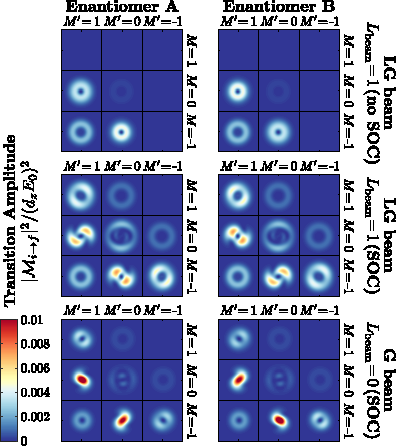
\includegraphics[width=1.0\columnwidth]{Figure2.pdf}
    \caption{由拉盖尔-高斯光束耦合的对映异构体在$\bra{1_{1,1}(M)}$到$\ket{1_{0,1}(M')}$跃迁的\eoet 信号剖面图,其中顶部为无自旋轨道耦合情况,中间行包含自旋轨道耦合,底部为高斯光束结合自旋轨道耦合的情况。}
    \label{fig:profiles}
\end{figure}
首先注意到,除非$d_zQ_{xy}^*$存在虚部${\rm Im}[d_zQ_{xy}^*]$,否则所有分布曲线的积分值相等。虚部会导致总吸收水平的二色性,这是已知的振动CD来源,其仅取决于分子内部参数而与电场结构无关(见\cite{Buckingham1971})。由此得出结论:仅通过光吸收强度无法检测HD,必须借助吸收剖面的空间分辨\cite{Loeffler2011}。

若无光SOC,两个对映体间唯一差异是$M=0\to M'=1$与$M=-1\to M'=0$剖面的强度(图~\ref{fig:profiles}顶行)。该二色性源于光束的$m=0$分量——即图~\ref{fig:gridJ1}中$\sigma=-1$、$m=0$面板虚线框内的红蓝方框,因此这是另一种空间分辨振动CD来源(无OAM转移)。

聚焦场引入的光SOC导致吸收剖面出现新的对映体区分效应(图~\ref{fig:profiles}中行)。首先,$M=-1\to M'=0$与$M=0\to M'=1$跃迁的吸收存在显著差异。该信号源自图~\ref{fig:gridJ1}虚线框内偶极与四极跃迁的耦合。这种差异源于涡旋光束与手性分子的相对螺旋性,并涉及OAM转移,因此可视为真正的HD。
此外,$M=1\to M'=1$与$M=-1\to M'=-1$的谱线轮廓也存在差异。这源于虚线框中$\sigma=0$的偶极跃迁(图~\ref{fig:gridJ1})与$m=-1$、$\sigma=-1$方框中四极跃迁的耦合作用,因此同样属于螺旋二色性(HD)。总体而言,自旋轨道耦合(SOC)光作用下的二色性信号强度比无耦合情况高出一个数量级。

图\ref{fig:profiles}最下行表明,在SOC条件下无需使用携带轨道角动量(OAM)的渐进极限光束。事实上,紧聚焦高斯光束同样能观测到HD现象。这是因为焦场会形成方位角电荷为$\sigma$的拉盖尔-高斯(LG)模式。更值得注意的是,紧聚焦的线偏振光束也会产生类似二色性,因为其内部两个圆偏振分量会通过SOC发生耦合。这说明入射光束的OAM或自旋并非观测HD的必要条件,真正的关键因素在于SOC效应。

需要强调的是,由于光子的SOC效应,分子所吸收的角动量类型难以明确区分,这导致我们无法简单地将产生的二色性归类为圆二色性(CD)或螺旋二色性(HD)。我们的工作通过量子数$m$和$\sigma$(见图~\ref{fig:profiles})明确了OAM与自旋的吸收通道,为解决该问题提供了方案。

综上所述,我们证明了傍轴OAM光束无法产生HD——这些条件下观测到的二色性均可归约为标准CD。真正的HD(与OAM转移直接关联的二色性)需要光的自旋-轨道耦合,例如在紧聚焦光束中。引人注目的是,即使高斯模式在远场不携带OAM,经充分聚焦后仍可展现本征HD。这些发现阐明了结构光实验中HD的起源,并提示先前关于HD的测量结果可能需要重新审视以确认OAM转移的存在。特别值得注意的是,未观测到二色性的研究要么主要探测偶极级相互作用\cite{Araoka2005},要么因信号平均化导致二色性消失\cite{Loeffler2011};而成功检测到二色性的研究均同时利用了四极场相互作用和紧聚焦光束\cite{Rusak2019,Rouxel2022,Begin2023,Jain2023}。

本文建立的框架为设计基于光场空间结构的 chiral-sensitive 光谱学和 enantiomer 分离方法提供了路线图~\cite{Leibscher2022}。\\
\begin{acknowledgments}
本研究全部或部分由奥地利科学基金(FWF)资助[项目编号:10.55776/F1004]。
\end{acknowledgments}
\bibliography{bibliography}
\end{CJK*}
\end{document}
